
%(BEGIN_QUESTION)
% Copyright 2010, Tony R. Kuphaldt, released under the Creative Commons Attribution License (v 1.0)
% This means you may do almost anything with this work of mine, so long as you give me proper credit

A chemical process typically operating at a pressure of 550 PSI occasionally experiences momentary pressure ``spikes'' in excess of 900 PSI.  These are transient events, never lasting more than a few seconds at a time.  A PLC receives a discrete signal from a pressure switch set to trip at 850 PSI:

$$\includegraphics[width=15.5cm]{i03510x01.eps}$$

Examine the RLL (Relay Ladder Logic) program in this PLC, and describe how the program is supposed to function.  Note that the timer instruction used here is {\it non-retentive}:

$$\includegraphics[width=15.5cm]{i03510x02.eps}$$

\underbar{file i03510}
%(END_QUESTION)





%(BEGIN_ANSWER)

This program turns on the lamp if there are 17 or more overpressure events in an hour of time.

%(END_ANSWER)





%(BEGIN_NOTES)

{\bf This question is intended for exams only and not worksheets!}.

%(END_NOTES)

